% Supplementary appendices: material moved out of the paper's appendix (the calibrated time model, the grid of
% other cards, and the accounting of the gap as a model). Built into supplement.tex, with references into
% the paper resolved from paper.aux.
\section{The calibrated time model}\label{app:law}
Our cache's one per-machine decision, how many of a layer's misses to fetch rather than run on the CPU, comes from a
calibrated model of time per token. With $X_c$ the bytes the CPU reads per token and $X_p$ the bytes the link reads,
\begin{equation}
T \;=\; G_{\mathrm{fit}} \;+\; \max\!\Big(\frac{X_c}{B_c},\ \frac{X_p}{B_p},\ \frac{X_c+X_p}{B_{cp}}\Big),
\label{eq:law}
\end{equation}
with one constant $G_{\mathrm{fit}}$ per engine and model, fitted once on one host and frozen (it is neither the profiled
$G$ of \cref{eq:sum} nor $T_{\text{GPU}}$ of \cref{eq:demand}). It is a calibrated model, not a law: $G_{\mathrm{fit}}$ is
fitted, and it exceeds the whole all-in-VRAM token (\lawGRefit{} against \vramMs\,ms) because it absorbs
per-token host work and the CPU helpers' shortfall against the probe (below). As a predictor of time it ties a naive
one-path model with the same $G_{\mathrm{fit}}$ (time $= G_{\mathrm{fit}} +$ all host bytes over the best probed rate):

\begin{center}\small
\begin{tabular}{lrrrr}\toprule
Held-out set & \multicolumn{2}{c}{\cref{eq:law}} & \multicolumn{2}{c}{one path} \\
 & median & 90th pct. & median & 90th pct. \\\midrule
blind test, \lawRows{} rows on \lawHosts{} hosts & \lawRowsMedian\% & \lawRowsPninety\% & \lawNaiveMed\% & \lawNaivePninety\% \\
frozen, \lawFrozenN{} rows on \lawFrozenHosts{} later hosts & \lawFrozenMed\% & \lawFrozenPninety\% & \lawFrozenNaiveMed\% & \lawFrozenNaivePninety\% \\
\bottomrule\end{tabular}
\end{center}
It over-predicts Qwen3's speed on the later hosts by \lawFrozenQwenMin{} to \lawFrozenQwenMax\%, a budget-dependent
bias whose $G_{\mathrm{fit}}$ was borrowed from llama.cpp. Its value is the per-machine fetch table it picks (\cref{eq:split} below),
which gains \lawGainMin--\lawGainMax\% over a fixed table on host B and \hpQwenLawMin--\hpGptLawMax\% on hosts with half
the link (\cref{app:system}).

\paragraph{The blind test in full.} On every machine of the blind test the job wrote the model's prediction from its own
probe before any model ran (\cref{tab:law}; all of its cache rows are gpt-oss-120b on RTX 5090 hosts). Over
\lawCfg{} configurations on \lawHosts{} machines (\lawMeas{} measurements; one machine ran twice) the median error is
\lawMedian\% per configuration; without the 12-channel EPYC 9655 it is \lawDeskMedian\% over \lawDeskN{}
configurations (90th percentile \lawDeskPninety\%). llama.cpp \texttt{--n-cpu-moe} is predicted within 4\% on the
Ryzen hosts, including two Qwen3 configurations on host B (+3.6\%, +4.0\%; for Qwen3, $G_{\mathrm{fit}}{=}4.3$\,ms, the mean
residual of three llama.cpp runs on another host), and misses by \lawLlamaOffMin--\lawLlamaOffMax\% on the
hybrid-core and server hosts. With its constants frozen, the model scores the cache on the \lawFrozenHosts{} RTX 5090
hosts rented later (\lawFrozenN{} measurements at the six cells of \cref{tab:headline}, not written before the runs)
at a median \lawFrozenMed\%, 90th percentile \lawFrozenPninety\%, worst \lawFrozenMax\% (\lawFrozenWorstCell).
Refit under leave-one-host-out validation, the token-level max has a median error of \lohoMaxMed\% (90th percentile
\lohoMaxPninety\%), the additive form $G_{\mathrm{fit}}+X_c/B_c+X_p/B_p$ \lohoAddMed\% (\lohoAddPninety\%) and a per-layer max summed
over layers \lohoLayerMed\% (\lohoLayerPninety\%); the max beats the sum on the three rows that copy misses on
demand behind a 53\,GB/s link, where both paths carry most of the bytes, and on the EPYC 9655 rows, where both fail,
the sum is closer on the two rows that copy behind a slow link, and elsewhere the two are within a few points
(\cref{app:law}). Each failure has a
measured cause (\cref{app:law}): on-demand copies behind a slow link share DRAM less evenly than the probe's combined
rate says; llama.cpp splits every matrix evenly across threads and runs at 46\% of the model on a hybrid-core host; and
on a 12-channel EPYC host memory stops being the limit and a per-layer latency floor takes over. $G_{\mathrm{fit}}$
(\lawGRefit\,ms refit) exceeds the whole all-in-VRAM token (\vramMs\,ms) because it absorbs a shortfall the probe does
not see: the helpers read at \helperRateMin--\helperRateMax$\times$ the probe's time per expert, and a fitted rate
factor is collinear with $G_{\mathrm{fit}}$ at this sample size.

\begin{table}[t]\centering\small
\caption{The law predicted blind: each machine wrote its prediction from its own bandwidth probe, with constants frozen
in the public repository, before any model run. Error of predicted over measured speed, gpt-oss-120b (cache rows) and
llama.cpp \texttt{--n-cpu-moe} (last column, \%).}\label{tab:law}
\setlength\tabcolsep{3pt}\resizebox{\linewidth}{!}{%
\begin{tabular}{llrrrl}\toprule
Host CPU & Job & $n$ & Median & Max & llama.cpp \\
 & & & $|$err$|$ \% & $|$err$|$ \% & err \% \\\midrule
Core Ultra 7 270K (8P+16E) & 069c & 5 & 1.5 & 11.9 & +119 \\
EPYC 7352 (Zen 2) & 069c & 5 & 3.2 & 11.7 & +10 \\
EPYC 9655 (12-ch.\ DDR5) & 069c & 5 & 18.7 & 31.9 & +16 \\
Ryzen 9 7900 & 072 & 5 & 4.9 & 8.2 & +4 \\
Ryzen 9 9950X3D (A) & 073 & 8 & 1.6 & 4.5 & -- \\
Ryzen 9 7950X & 074 & 1 & 4.0 & 4.0 & -- \\
Ryzen 9 9950X & 076 & 4 & 2.5 & 5.0 & -- \\
Ryzen 9 9950X3D (B) & 082 & 0 & -- & -- & +4, +4 \\
\bottomrule\end{tabular}}\end{table}


\paragraph{What the model says, and the split it picks.} \Cref{eq:law} is a calibrated model of execution that reads host
memory in sequence with its GPU work, as our cache and llama.cpp do. For such an engine every mechanism acts only
through the bytes read from host memory per token and the number of read paths in use: a second path adds bandwidth on
every host of the blind test but the 12-channel EPYC ($B_{cp}$ against $\max(B_c,B_p)$: \secondMin--\secondMax\%
on its Ryzen hosts, \secondUltra\% on the Core Ultra, \secondEpyc\% on the Zen~2 EPYC; the RTX 3090 host's Core
i9-11900KF, where the two paths together read less than the CPU alone, is a second exception), and that is the whole
gain available to fetching or splitting misses between the CPU and PCIe. Prefetching never reduces the bytes; what
it can buy is overlap of the reads with the step, which the model does not price: charging every read in sequence, it
over-predicts the time per token of the read-ahead oracle by \fxPacedLawTimeMin{} to \fxPacedLawTimeMax\% (\cref{sec:foresight})
and of a Belady prefetch by up to \fspLawErrHighMax\% (\cref{app:foresight}). The model's job in the system is the split.
Its
per-layer form,
\begin{equation}
T(n,f)=\max\!\big(\tfrac{fS}{B_p}+g,\ [n{>}f](L_c+\tfrac{(n-f)S}{B_c}),\ [0{<}f{<}n]\tfrac{nS}{B_{cp}}\big),
\label{eq:split}
\end{equation}
with $g$ the GPU's expert work per layer (48\,$\mu$s for Qwen3, 37\,$\mu$s for gpt-oss, from profiles) and
$L_c{=}20\,\mu$s the hand-off, picks for each count $n$ of missed experts the number $f$ to copy with the smallest
$T$. On host B the model's table beats the fixed table we used before at every budget of both models, by
\lawGainMin--\lawGainMax\%; on hosts whose link we measured at 27--30\,GB/s instead of 53 it fetches less and gains
\hpGptLawMin--\hpGptLawMax\% on gpt-oss and \hpQwenLawMin--\hpQwenLawMax\% on Qwen3, the per-machine split mattering
most where the link is slow (\cref{app:system}). In the running example on host B the table is
\texttt{\scTableGptB} ($f(0..4)$): one missed expert runs on the CPU, hidden behind the GPU's other experts; from two
misses the model copies one. The lead over FreeToken at that cell, \ftRatioGptMid$\times$, is mostly the admission
policy (\scPolicyShareGptMin\% of it by the LRU ablation of \cref{app:system}), the rest the CPU path that FreeToken's
bandwidth model declines to use there.

\paragraph{Is the max the right form?} In 19 of the \lawCfg{} configurations nothing is copied, so they test one
roof. We therefore refit the model and its alternatives on the same \lawRows{} measurements under leave-one-host-out
validation (each of the \lawHostsLoho{} hosts predicted with constants fitted on the other \lawHostsLohoOther): the token-level max of
\cref{eq:law} with $G_{\mathrm{fit}}$ refit has a median error of \lohoMaxMed\% (90th percentile \lohoMaxPninety\%); the additive form
$G_{\mathrm{fit}}+X_c/B_c+X_p/B_p$, \lohoAddMed\% (\lohoAddPninety\%); a per-layer max summed over layers from the engine's per-layer
miss histograms, \lohoLayerMed\% (\lohoLayerPninety\%). The additive form ties in sample but misses the three
rows that copy misses on demand behind a 53\,GB/s link, where both paths carry most of the bytes, by
\lohoAddFastFetchMin\%, while the max is within $\pm$0.2\% there; on the slow-link copy rows the additive form is the
closer of the two. The per-layer form neither beats the max nor explains its failures: the Jensen gap between a sum
of per-layer maxima and the maximum of sums is a fifth of the Core Ultra's residual, none of the EPYC 7352's, and has
the wrong sign on the EPYC 9655 and on the prefetch rows. We keep \cref{eq:law}, with its evidence stated: the max beats the sum on the three fast-link copy rows and on the
EPYC 9655 rows, where both fail, the sum is closer on the two slow-link copy rows, and elsewhere the two are within a
few points, so the form is settled only where both paths carry most of the bytes. FreeToken's own runs are not
predicted, because its counters are not exposed; the model covers our engine and llama.cpp.

\paragraph{Where it fails, and why.} Each failure now has a measured cause. (i) Copying misses on demand (FETCH) at
25\% is over-predicted by \lohoFrozenFetchUltra\% on the Core Ultra 7 and \lohoFrozenFetchEpyc\% on the EPYC 7352 (links
of 36 and 26\,GB/s); \lohoMaxFetchUltra\% and \lohoMaxFetchEpyc\% with $G_{\mathrm{fit}}$ refit. The engine's per-layer timers show
why: a CPU miss served beside a copy takes \fetchBesideMin--\fetchBesideMax\% longer than one served alone, so the two
paths share DRAM less evenly than the probe's combined rate says; a variant of the model that uses the probe's
per-path rates under contention and a per-layer hand-off constant predicts both rows within \lohoAsymFetchUltra\% and
\lohoAsymFetchEpyc\%, at a worse median (\lohoAsymMed\%). (ii) llama.cpp on a Core Ultra 7 with 8 performance and 16 efficiency cores runs at 46\% of the
model's prediction at its default thread count, because it splits every matrix evenly across its threads; our helpers claim work
dynamically and stay on the model on the same machine. We did not test llama.cpp restricted to the performance cores.
(iii) On a 12-channel EPYC 9655 (559\,GB/s) host memory stops being the limit (\lohoMaxEpycMin{} to
\lohoMaxEpycMax\% with $G_{\mathrm{fit}}$ refit under leave-one-host-out validation; \cref{tab:law} gives the blind errors): the per-layer timers show a floor of \epycFloorMin--\epycFloorMax\,$\mu$s per layer with CPU misses
that no desktop host has (their intercepts are at or below zero), the latency of the hand-off at a bandwidth where a
13\,MB expert takes 24\,$\mu$s. (iv) Prefetch configurations are under-predicted by \lohoMaxPfMin{} to
\lohoMaxPfMax\%: their copies overlap attention, which the model charges in full.

\section{The grid: other cards, and the scope of the gain}\label{app:grid}
\begin{figure}[t]\centering
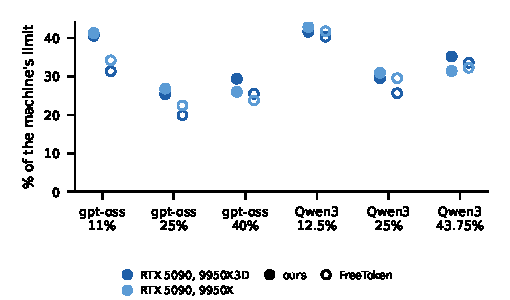
\includegraphics[width=0.5\linewidth]{figs/grid.pdf}
\caption{Ours (filled) and FreeToken (hollow) as a percentage of each machine's own bound (exact optimum,
the machine's highest probed host rate, the card's datasheet rate) at every cell of \cref{tab:grid}: two RTX 5090
hosts, an RTX 4090 and an RTX 3090 (FreeToken's 3090 cells, its carried-over backend running below llama.cpp, are
omitted). The limit ranges from \grLimMin{} to \grLimMax\,tok/s across these cells; ours stays at
\grFracMin--\grFracMax\% of it.}\label{fig:grid}
\end{figure}
\Cref{tab:grid} lists every cell of \cref{tab:headline}'s protocol on the four machines we measured, each against its
own limit, and \cref{fig:grid} plots the fractions. The protocol was repeated on an RTX 4090 next to a Core i5-12400
(the host reads \grFourkHostBw\,GB/s, the link 25) and an RTX 3090 next to a Core i9-11900KF (\grThreekHostBw\,GB/s;
CPU and link together read \emph{less} than the CPU alone, so the model's table copies nothing), at the cells that fit
24\,GB. On the 4090 ours runs \grFourkFtMin--\grFourkFtMax$\times$ FreeToken and
\grFourkLlamaMin--\grFourkLlamaMax$\times$ llama.cpp at half host B's absolute speeds, the host being the reason; on
the 3090 it runs \grThreekLlamaMin--\grThreekLlamaMax$\times$ llama.cpp (FreeToken's carried-over backend ran below
llama.cpp there and is not counted). The cards' own bandwidth never enters: \grSmallHostBound{} one of the
\grSmallCellsN{} cells on the 24\,GB cards is host-bound at the limit, and ours stands at
\grFourkFracMin--\grFourkFracMax\% and \grThreekFracMin--\grThreekFracMax\% of it. Mixtral-8x7B (8 experts per layer,
top-2; 26\,GB of experts on the 3090) marks the scope: with 2 of 8 experts resident the cache hits \grMixHitCTwo\% of
reads where whole-layer pinning hits \grMixPinCTwo\%, so there is little locality to earn, and ours ties llama.cpp
(\grMixCTwo{} [\grMixCTwoLo, \grMixCTwoHi]); on the 128-expert models the same cache hits \grHitMin--\grHitMax\% at
11--25\% resident. Across \ratioHostsN{} hosts the gpt-oss lead over FreeToken grows with the host's CPU-to-link
ratio, from \ratioNearMin--\ratioNearMax$\times$ where the CPU reads \ratioNearXMin--\ratioNearXMax$\times$ its link's
rate to \slFtMin--\slFtMax$\times$ behind a link of half the bandwidth, in the direction the model's split implies
(the model does not predict FreeToken's runs), and the Qwen3 lead stays
at \ratioQwenLo--\ratioQwenHi$\times$ (\cref{fig:ratio}, \cref{app:system}).

\begin{figure}[t]\centering
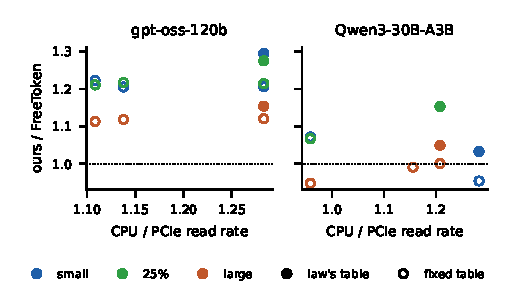
\includegraphics[width=0.5\linewidth]{figs/ratio.pdf}
\caption{Ours over FreeToken's better backend (carried over from host B on host S) in every same-machine comparison
of the current engine on the two models of \cref{tab:headline} (\ratioHostsN{} hosts), against the machine's
CPU-to-PCIe read ratio (FreeToken's own probe). Filled: FETCH table from the model on that machine; hollow: the fixed
table. The rightmost gpt-oss points are a Core i9-14900K with FreeToken's executor on its performance cores; the
rightmost Qwen3 points are a Ryzen 9 7900.}\label{fig:ratio}
\end{figure} The 24\,GB cards run the cells
that fit (the VRAM arithmetic, written on the machine from the GGUF header, skipped Qwen3 at 43.75\%: 28.0\,GB of
slots, dense weights and KV against a 23\,GB limit). The predictions for jobs 091 and 092 and their outcomes are in
\texttt{prereg/grid\_outcome\_091.md} and \texttt{092.md}: on the 4090 our lead over FreeToken at gpt-oss 11\% (37\%)
exceeded the predicted 10--35\% band, ours ran 1.78$\times$ llama.cpp at Qwen3 12.5\% against a predicted 1.8, the model's
tables copied one more expert than host B's at one entry each (the prediction reasoned from the link
alone; the CPU is slower in the same proportion), and ours' fraction of the limit at Qwen3 12.5\% (45.7\%) exceeded the
predicted 25--45\%; on the 3090 FreeToken's carried-over backend ran below llama.cpp, ours ran 1.56--1.64$\times$
llama.cpp at two cells against a predicted 1.8, Mixtral tied at $C{=}2$ against a predicted 1.3$\times$ and its
$C{=}4$ cell was lost to the job's deadline, and one launch-order check exceeded 3\% (7\%).

\begin{table*}[t]\centering\small
\caption{The grid: \cref{tab:headline}'s protocol on every card and host we measured, each cell against its own
machine's limit (the exact optimum's reads on the same trace, the machine's highest probed host rate, the card's
datasheet rate). \emph{Bound}: what binds the limit; \emph{host} when the optimum's reads alone take longer than the
GPU's whole read, so the GPU has slack, \emph{both} when the limit runs experts on the CPU until the two paths take
equally long, which is where the all-in-VRAM speed can be exceeded. Ours and
FreeToken are launch 2 (FreeToken's backend carried over from the headline machine's selection); the 40 and 43.75\%
budgets do not fit a 24\,GB card. Mixtral-8x7B (26\,GB of experts, top-2 of 8) is ours against llama.cpp only, on the
RTX 3090, launch 1.}\label{tab:grid}
\setlength\tabcolsep{3pt}\resizebox{\textwidth}{!}{%
\begin{tabular}{llrrrcrrcr}\toprule
Model & Experts & llama.cpp & FreeToken & Ours & Ours $\div$ FreeToken & Ours $\div$ & Limit & Bound & Ours, \% \\
 & on GPU & (tok/s) & (tok/s) & (tok/s) & (95\% CI) & llama.cpp & (tok/s) & & of limit \\
\midrule
\multicolumn{10}{l}{\textbf{RTX 5090}, 9950X3D (listing B): $B_{\mathrm{host}}$ 88\,GB/s, $B_{\mathrm{gpu}}$ 1792\,GB/s; tables \texttt{0,0,1,1,2} / \texttt{0,0,1,1,2,3,3,4,5}} \\
gpt-oss-120b & 11\% & 34.9 & 54.0 & 69.9 & 1.29 [1.28, 1.31] & 2.00 & 172 & host & 41 \\
gpt-oss-120b & 25\% & 40.0 & 85.6 & 109.2 & 1.27 [1.25, 1.29] & 2.73 & 430 & host & 25 \\
gpt-oss-120b & 40\% & 47.7 & 132.2 & 152.5 & 1.15 [1.13, 1.17] & 3.20 & 519 & both & 29 \\
Qwen3-30B-A3B & 12.5\% & 19.5 & 38.7 & 40.0 & 1.03 [1.02, 1.04] & 2.05 & 96 & host & 42 \\
Qwen3-30B-A3B & 25\% & 22.1 & 54.7 & 63.1 & 1.15 [1.13, 1.17] & 2.86 & 214 & host & 30 \\
Qwen3-30B-A3B & 43.75\% & 28.4 & 103.1 & 108.2 & 1.05 [1.04, 1.06] & 3.81 & 308 & both & 35 \\
\midrule
\multicolumn{10}{l}{\textbf{RTX 5090}, 9950X (job 089): $B_{\mathrm{host}}$ 71\,GB/s, $B_{\mathrm{gpu}}$ 1792\,GB/s; tables \texttt{0,0,1,2,3} / \texttt{0,0,1,2,2,3,4,5,6}} \\
gpt-oss-120b & 11\% & 28.9 & 48.0 & 57.9 & 1.21 [1.19, 1.22] & 2.00 & 140 & host & 41 \\
gpt-oss-120b & 25\% & 33.6 & 78.7 & 94.1 & 1.20 [1.16, 1.22] & 2.80 & 351 & host & 27 \\
gpt-oss-120b & 40\% & 40.1 & 122.2 & 133.6 & 1.09 [1.08, 1.11] & 3.34 & 514 & both & 26 \\
Qwen3-30B-A3B & 12.5\% & 16.1 & 32.7 & 33.5 & 1.03 [1.02, 1.04] & 2.08 & 78 & host & 43 \\
Qwen3-30B-A3B & 25\% & 18.5 & 51.4 & 53.9 & 1.05 [1.04, 1.06] & 2.91 & 174 & host & 31 \\
Qwen3-30B-A3B & 43.75\% & 23.8 & 98.3 & 95.8 & 0.97 [0.96, 0.99] & 4.02 & 305 & both & 31 \\
\bottomrule\end{tabular}}\end{table*}


\section{The order-free accounting of the gap}\label{app:accounting2}
% generated by scripts/factorial_shapley.py
\begin{table*}[t]\centering\footnotesize
\caption{An order-free accounting of the gap between the deployed cache and the bound at the host-bound budgets, as
percentages of the gap (ms per token). The engine ran both choices of what to cache (the deployed policy's admissions
or MIN's) with both ways to load a cached expert (two reads: the CPU serves it, then a copy; one read: a copy in the
step). \emph{Load alone} and \emph{cache alone} are each choice's effect with the other at the deployed level; the
\emph{interaction} is how much more MIN's set is worth loaded once than loaded twice. The Shapley values average each
choice's effect over the other's two levels and add up, with the prefetch (nested under MIN's set, since it needs
foresight) and the rest, to 100\%. Panel: mean over its hosts (number
in parentheses) and, in small type, the range over its hosts (not an interval); a fast link reads at least half as fast as
the host's CPU, a slow one less. Last rows: the new machines of the follow-up launches, with their link-to-CPU ratio.}\label{tab:shapley}
\setlength\tabcolsep{3pt}\resizebox{\textwidth}{!}{%
\begin{tabular}{llrrrrrrrr}\toprule
 & & Gap & Load & Cache & Inter- & \multicolumn{2}{c}{Shapley value} & Prefetch & Rest \\
Host & Budget & (ms) & alone & alone & action & cache & load & & \\\midrule
O4 & gpt-oss 11\% & 10.6 & 4 & 4 & 43 & 26 & 25 & 13 & 36 \\
O4 & gpt-oss 25\% & 8.5 & 4 & 22 & 17 & 31 & 13 & 22 & 34 \\
O4 & Qwen3 12.5\% & 18.4 & 3 & $-$1 & 58 & 28 & 32 & 4 & 36 \\
O4 & Qwen3 25\% & 14.1 & 2 & 14 & 37 & 33 & 21 & 17 & 30 \\
O5 & gpt-oss 11\% & 11.4 & 0 & $-$2 & 28 & 12 & 14 & 17 & 57 \\
O5 & gpt-oss 25\% & 9.1 & $-$4 & 20 & 10 & 25 & 1 & 21 & 52 \\
O5 & Qwen3 12.5\% & 19.8 & 1 & $-$13 & 43 & 9 & 23 & 7 & 62 \\
O5 & Qwen3 25\% & 15.3 & 0 & 14 & 17 & 22 & 9 & 16 & 53 \\
\midrule
Panel, fast link (8) & gpt-oss 11\% & 11.6 & 1 {\scriptsize($-$2 to 4)} & 3 {\scriptsize($-$2 to 6)} & 38 {\scriptsize(30 to 47)} & 22 {\scriptsize(14 to 26)} & 20 {\scriptsize(14 to 27)} & 13 {\scriptsize($-$4 to 20)} & 45 {\scriptsize(38 to 55)} \\
Panel, fast link (8) & gpt-oss 25\% & 9.0 & 0 {\scriptsize($-$4 to 3)} & 22 {\scriptsize(18 to 26)} & 15 {\scriptsize(10 to 19)} & 29 {\scriptsize(25 to 35)} & 8 {\scriptsize(1 to 12)} & 20 {\scriptsize(9 to 23)} & 43 {\scriptsize(38 to 49)} \\
Panel, slow link (2) & gpt-oss 11\% & 9.7 & $-$6 {\scriptsize($-$9 to $-$3)} & $-$4 {\scriptsize($-$9 to 0)} & 3 {\scriptsize($-$6 to 11)} & $-$3 {\scriptsize($-$11 to 6)} & $-$5 {\scriptsize($-$12 to 2)} & 17 {\scriptsize(9 to 24)} & 91 {\scriptsize(83 to 99)} \\
Panel, slow link (2) & gpt-oss 25\% & 7.8 & $-$17 {\scriptsize($-$22 to $-$11)} & 19 {\scriptsize(16 to 23)} & 3 {\scriptsize(3 to 3)} & 21 {\scriptsize(17 to 25)} & $-$15 {\scriptsize($-$21 to $-$10)} & 22 {\scriptsize(17 to 26)} & 73 {\scriptsize(68 to 78)} \\
\midrule
5700X3D (0.92) & gpt-oss 11\% & 14.9 & 4 & $-$2 & 55 & 25 & 31 & 8 & 36 \\
5700X3D (0.92) & gpt-oss 25\% & 11.5 & 4 & 22 & 24 & 34 & 17 & 18 & 31 \\
9950X, x8 (0.54) & gpt-oss 11\% & 8.3 & 0 & $-$3 & 17 & 5 & 8 & 28 & 59 \\
9950X, x8 (0.54) & gpt-oss 25\% & 7.4 & $-$15 & 13 & 17 & 22 & $-$6 & 26 & 59 \\
9800X3D, slower link (0.61) & gpt-oss 11\% & 10.8 & $-$2 & $-$4 & 29 & 11 & 12 & 20 & 57 \\
9800X3D, slower link (0.61) & gpt-oss 25\% & 8.9 & $-$5 & 20 & 12 & 26 & 1 & 20 & 54 \\
\bottomrule\end{tabular}}\end{table*}


Two choices separate the deployed cache from MIN with one read: \emph{what to
cache} (the deployed policy's admissions or MIN's) and \emph{how to load} (by the CPU, two reads, or in the step, one).
The engine ran all four combinations on O4, O5, the panel and the three new machines of jobs 100--101. In the running example, changing only
what to cache closes \fsExSetTwo\% of the \fsExGap\,ms gap, changing only how to load \fsExReadsOnline\%, and both
\fsExBoth\% (rounded): the choices interact, because MIN caches \fxExAdmitsOverOnline{} times as many experts per token
as the deployed policy and, loaded by the CPU, each is read twice. We credit each choice with its effect averaged over
the two orders, its Shapley value \citep{fawcett2016ablation,jain1991art} (\fsExSet\% and \fsExReads\% here);
\cref{tab:shapley} also lists each alone and the interaction. Copying ahead is nested under MIN's set
(\fsExPacing\%); what no oracle touches is the rest (\fsExRest\%). On the \fsBalHosts{} hosts whose link reads at least
half as fast as the CPU, either change alone closes at most \fsBalAloneMax\% of the gap and both together
\fsBalBothMin--\fsBalBothMax\%; on the \fsSlowHosts{} below that line, loading in the step costs time at
\fsSlowReadsLoseN{} of \fsSlowCells{} host-budgets, and at \jeSlowReadsLoseN{} of \jeSlowCells{} on \jeSlowN{} more (job 103). These use the greedy set. With the fewest-admission set (job 104),
both together close \jfBothPlanLowMin--\jfBothPlanLowMax\% at 11\% on its three machines, against
\jfBothGreedyLowMin--\jfBothGreedyLowMax\% with the greedy set, and the interaction remains
(\jfInterPlanLowMin--\jfInterPlanLowMax\%).


\section{The accounting as a model}\label{app:accounting}
\begin{figure}[t]\centering
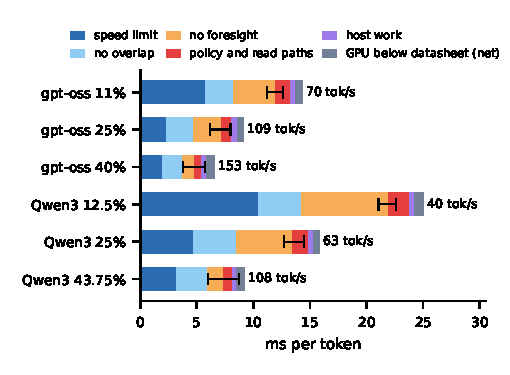
\includegraphics[width=\linewidth]{figs/shapley.pdf}
\caption{The accounting as a model: Shapley attribution of the gap between our cache's measured time per token and
the bound, for every cell of \cref{tab:headline} on host B, averaged over all \shOrders{} orders in which the
five fixes can be applied. Fixes: overlapping host reads with GPU work, which in \cref{eq:limit}'s form also moves
experts onto the CPU until the two paths balance; the optimum's reads instead of the best online policy's (foresight);
the best online policy's reads at the probe's highest rate instead of the engine's reads through \cref{eq:law}
(policy and read paths); the engine's per-token host work; and GPU kernels at the datasheet rate, the term that
closes the model on the measured time. Whiskers: the range of foresight's marginal cost over the orders.}
\label{fig:shapley}
\end{figure}

 Between the measured time of a cell and its limit lie five modelled fixes:
overlap of host reads with GPU work (in \cref{eq:limit}'s form, which also rebalances experts onto the CPU), the
optimum's reads instead of the online policy's (\emph{foresight}), the best online policy's reads at the probe's
highest rate instead of the engine's through \cref{eq:law} (policy and read paths), the engine's per-token host work,
and GPU kernels at the datasheet rate. Adding them in a fixed order makes the first one added look largest, so we
report each fix's Shapley value, its average marginal cost over every order (\cref{fig:shapley}), a method with a
precedent in performance debugging of microservices \citep{shapleyiq2024}. Two of the five terms are definitions
rather than measurements: the GPU term is the residual, its factor calibrated per cell so that the model with no fix
applied reproduces the measured time, and ``overlap'' is \cref{eq:limit}'s form. On host B the model has two regimes.
In the four host-bound cells missing foresight is the largest cost, \shFsHostMin--\shFsHostMax\% of the gap
(\shFsHostTokMin--\shFsHostTokMax\% of the token; in the running example \shFsGMid\%, where it edges overlap by
\shTieMs\,ms and is the largest marginal cost in \shOrdersGMid{} of the \shOrders{} orders); in the two GPU-bound cells
host reads serialised with GPU work is largest, \shOvlGpuMin--\shOvlGpuMax\% of the gap, and foresight second at
\shFsGpuMin\%. Policy and read paths cost \shPolMin--\shPolMax\%, per-token host work \shHostMin--\shHostMax\%, and
GPU kernels below datasheet, net of the overlap the engine achieves, \shGpuMin--\shGpuMax\%. The regimes are a
property of the host: recomputed for the three oracle hosts, whose host memory is weaker, foresight edges overlap at
three of their six GPU-bound cells. The model prices foresight and overlap as nearly independent players, and the
interior states it values are not realised by any online policy. The rest of this section measures them.

